\documentclass{article}
\usepackage{tikz}
\usepackage{pgfplots}
\pgfplotsset{compat=1.15} 

\begin{document}

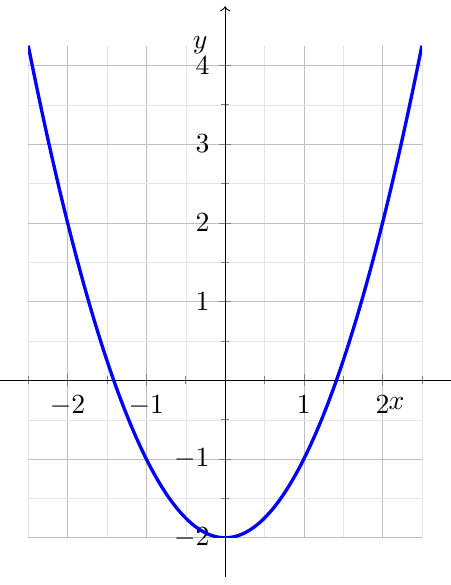
\begin{tikzpicture}
\begin{axis}[
    % 1. Genau 1cm pro Einheit (2 Kästchen = 1cm)
    x=1cm, y=1cm,
    xtick distance=1,    
    ytick distance=1,
    minor tick num=1,    
    grid=both,           
    major grid style={line width=.2pt,draw=gray!50},
    minor grid style={line width=.1pt,draw=gray!20},
    %
    % 2. Achsen in der Mitte
    axis lines=middle,
    %
    % VORLAGE FÜR WUNSCH 1: x-Label unter die Achse verschieben
    xlabel={$x$}, 
    xlabel style={at={(current axis.right of origin)}, anchor=north east, xshift=-0.1cm, yshift=-0.1cm}, 
    ylabel={$y$},
    ylabel style={at={(current axis.above origin)}, anchor=east, xshift=-0.1cm},
    %
    % VORLAGE FÜR WUNSCH 2: Graph bis an den Rand zeichnen
    enlargelimits=false, % Kein künstlicher weißer Puffer um den Graphen herum
    % Lässt NUR die Achsenlinien mit den Pfeilen 0.5cm (1 Kästchen) über den Rand des Rasters hinausragen:
    axis line style={->, shorten >=-0.5cm, shorten <=-0.5cm}, 
    %
    % Globale Einstellungen für die Kurve
    samples=150
]

% Deine Funktion: Zeichnet exakt von Anfang bis Ende des Rasters
\addplot[color=blue, very thick, domain=-2.5:2.5] {x^2 - 2};

\end{axis}
\end{tikzpicture}

\end{document}